\section{Overview}

\section{Structure}
	\subsection{Structure of an Individual Module}
		\subsection{Access to Other Simulation Elements}
		
The architecture of the simulator requires that communications modules are able to interact with the simulator environment (to dispatch messages), as well as with the messageable with which they are associated. Since it is impossible to have all of this information available when the communications module is instantiated (creating a messageable requires a reference to a communications module as well), it is necessary to set the messageable associated with a communications object at a later time (but before the simulation is started). Thus, the procedure for bootstrapping a simulations is broadly as follows:

\begin{enumerate}
	\item Load the sensor data
	\item Create a simulation environment referencing the sensor data
	\item Create a communications module referencing the environment
	\item Create a messageable referencing the environment and the communications module
	\item Add a reference to the messageable to the communications module
\end{enumerate}

How these references are used is covered in sections \ref{int-sim} and \ref{int-pro}.

		\subsubsection{Sending and Receiving Messages}
		
When a communications module wishes to transmit a message to other units it invokes the broadcast method exposed by the simulation environment. Messages that originate from the communication modules messageable collect in a queue, which must be checked at regular intervals. When there is a message that the environment determines should be delivered to the communications module, it is deposited in a similar queue. When the module has a message it needs to pass to its messageable, it stores it in a third queue.

In addition to asynchronous messaging, the project design also called for synchronous message passing. This is achieved by having a callback function in the messagable which can be invoked upon receipt of an urgent communication. It is left to the communication implementation to decide which messages are important to interrupt the normal operation of the messageable for.
		
		\subsubsection{Intermediate Processing}
		
	\subsection{Structure of a Collection of Modules}
	
In order to facilitate easy distribution and use, collections of communication implementations are combined into libraries. Given the small size of a communications modules source code (often tens of kilobytes) it might be tempting to statically link them to simulation executables. The problem with this approach, however, is that it precludes the very thing that prompted the creation of communications modules in the first place - modularity. As such, communications code is packaged into a shared library which simulator executables are then linked against dynamically at compile time. This reduces the size of produced executables and makes updating communications code possible without requiring simulations to be recompiled.

\section{Integration with Other Components}
	\subsection{Integration with the Simulator}
		\label{int-sim}
	\subsection{Integration with a Program}
		\label{int-pro}

\section{Provided Implementations}

\begin{figure}
\centering
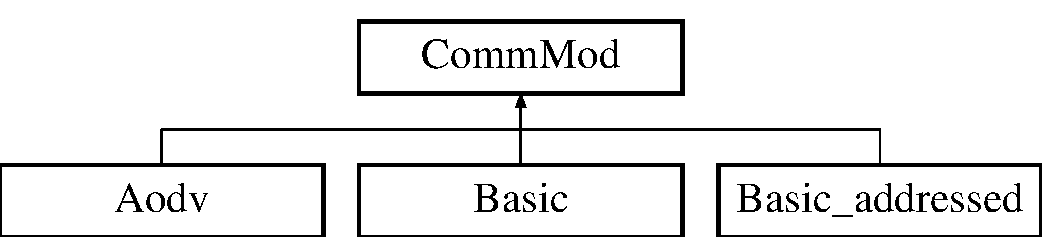
\includegraphics[scale=0.4]{../documentation/latex/class_comm_mod}	
\caption{Inheritance diagram for the \textit{CommMod} class}
\end{figure}

	\subsection{Basic Messaging}

\begin{figure}[H]
\centering
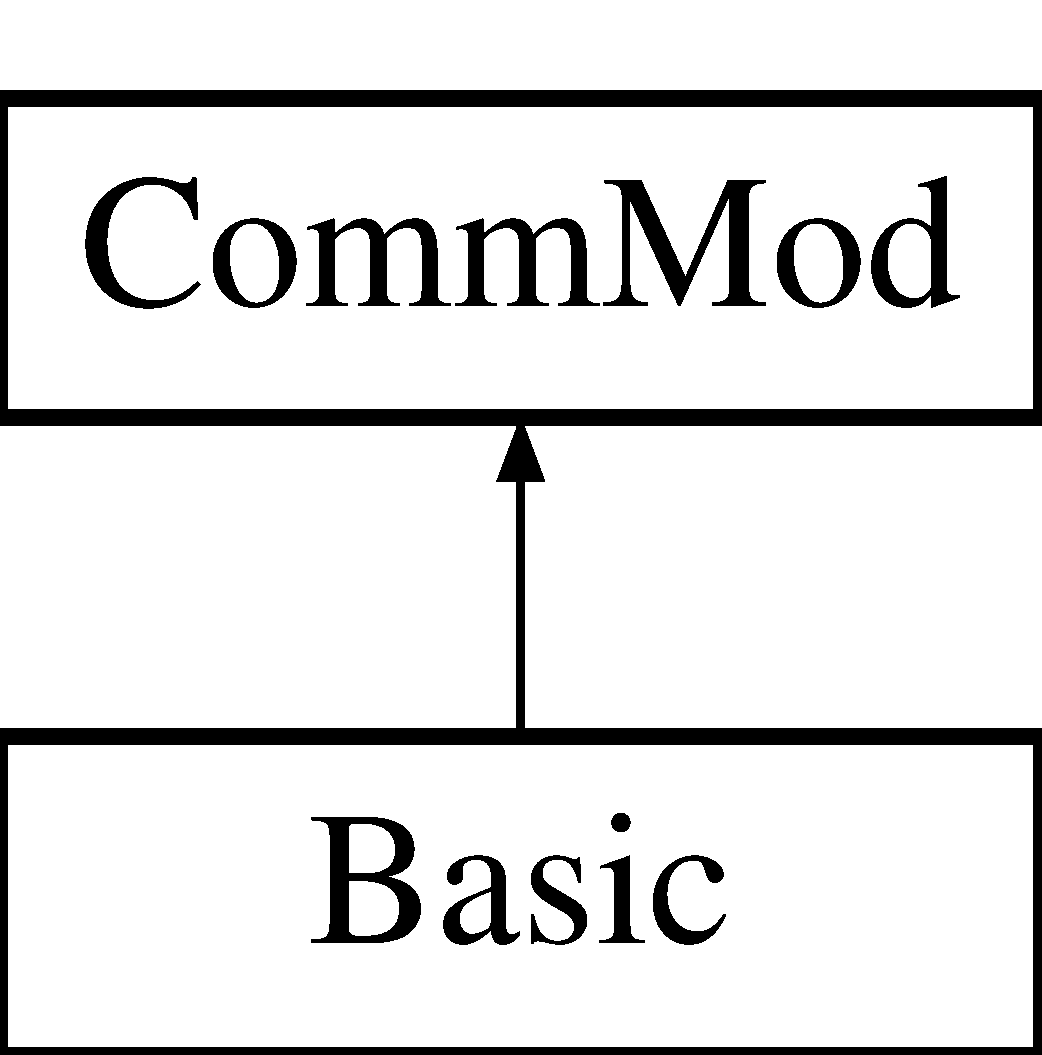
\includegraphics[scale=0.2]{../documentation/latex/class_basic}	
\caption{Inheritance diagram for the \textit{Basic} class}
\end{figure}
	
	\subsection{Addressed Basic Messaging}

\begin{figure}
\centering
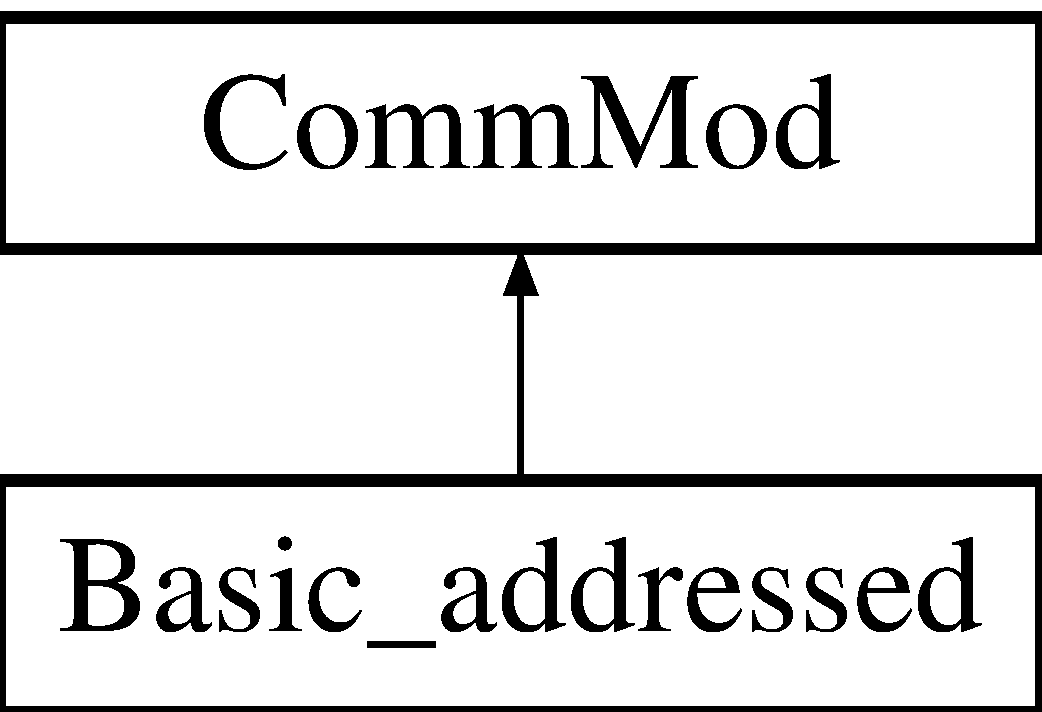
\includegraphics[scale=0.2]{../documentation/latex/class_basic__addressed}	
\caption{Inheritance diagram for the \textit{Basic\_addressed} class}
\end{figure}	
	
	\subsection{Ad hoc On-Demand Distance Vector Routing}

\begin{figure}
\centering	
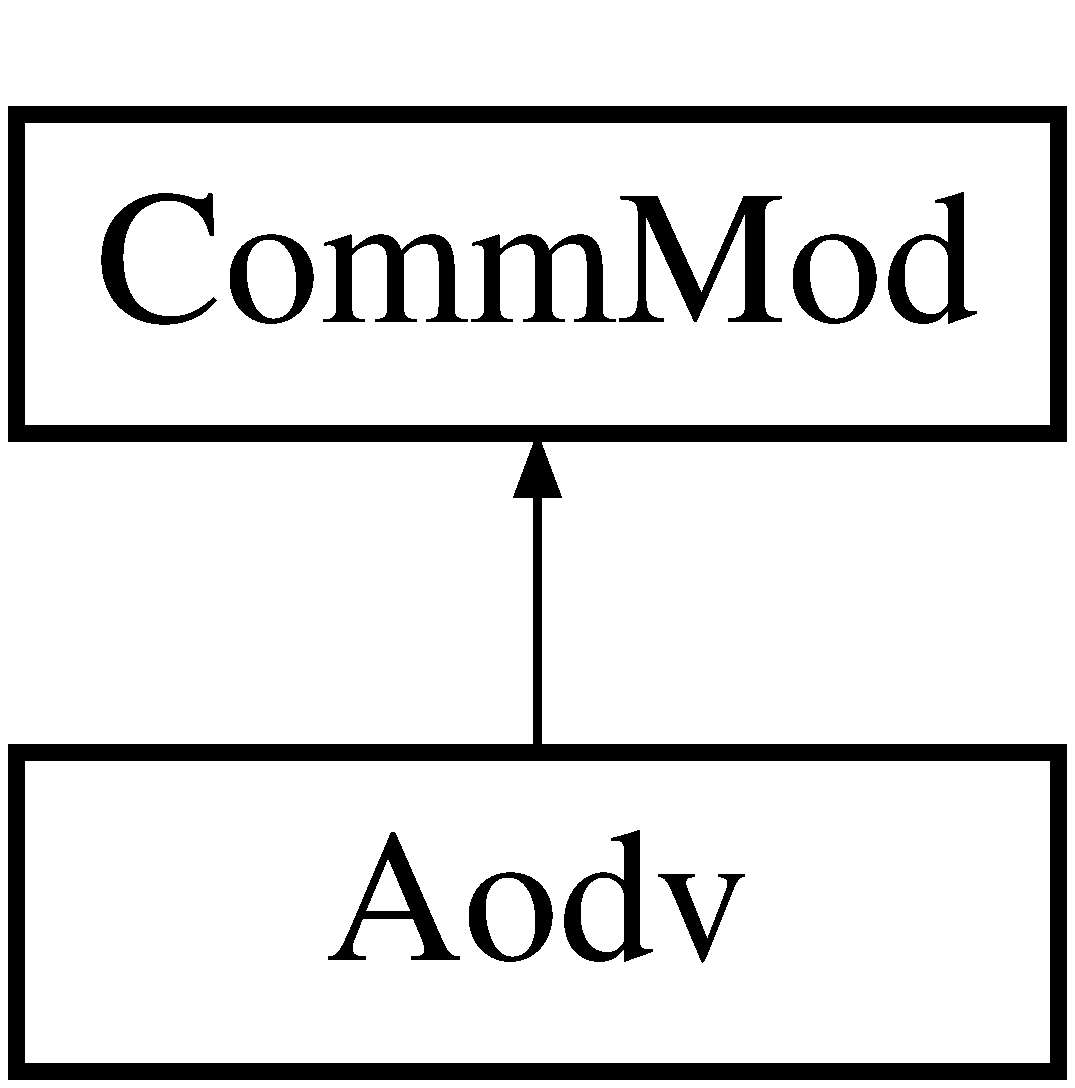
\includegraphics[scale=0.2]{../documentation/latex/class_aodv}	
\caption{Inheritance diagram for the \textit{Aodv} class}
\end{figure}